%!TEX root = ../../thesis.tex

\section{Detecting atmospheres}
\label{sec:decting_atmopsheres}
To help characterize an exoplanet, a detection of its atmosphere can provide useful information.
After the detection of exoplanets and the measurement of their bulk properties, detecting their atmospheres is the next step.
The detection of planetary atmosphere is difficult due to the low planet-to-star flux ratio.
This requires high precision instrumentation to detect.
For example the planet-to-star flux ratio in the optical is $\approx 10^{-4}$ for a hot Jupiter with a 3 day orbit, in which the main component is reflected star light.
In the infrared the thermal emission of the planet dominates and the flux ratio rises to $\approx 10^{-3}$.
These flux ratios requires observations with signal-to-noise ratios of $10^4$ and $10^3$ in the optical and infrared respectively to achieve a planetary signal at the same level as the noise level.
These detections are only just at the capabilities of the current generation of technology, and with very long observation cost.

Several photometric and high-resolution spectroscopic techniques are showing promising results; these are detailed in the following sections.


\subsection{Occultation and phase variations}
\label{subsec:phase_variation}

\begin{figure}
    \centering
    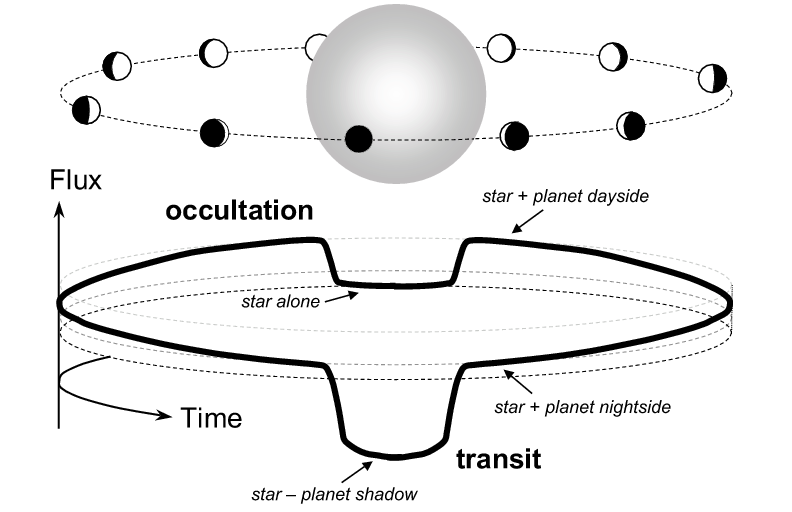
\includegraphics[width=0.6\linewidth]{./figures/introduction/circular_diagram.png}
    \caption[Flux contribution from a star and planet in a transiting exoplanet system.]{Illustration of the flux contribution from a star and planet in a transiting exoplanet system throughout its orbit.
    Credit~\citet{winn_transits_2010}.}
    \label{fig:transits_and_occultations}
\end{figure}

\begin{figure}
    \centering
    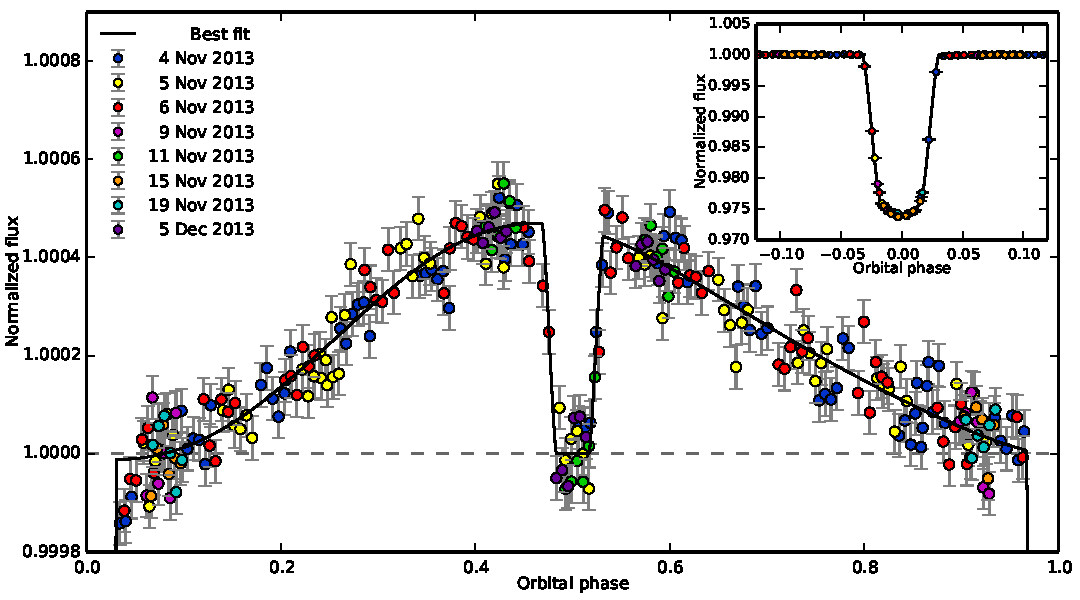
\includegraphics[width=0.5\linewidth]{figures/introduction/stevenson_phasecurve2014.pdf}
    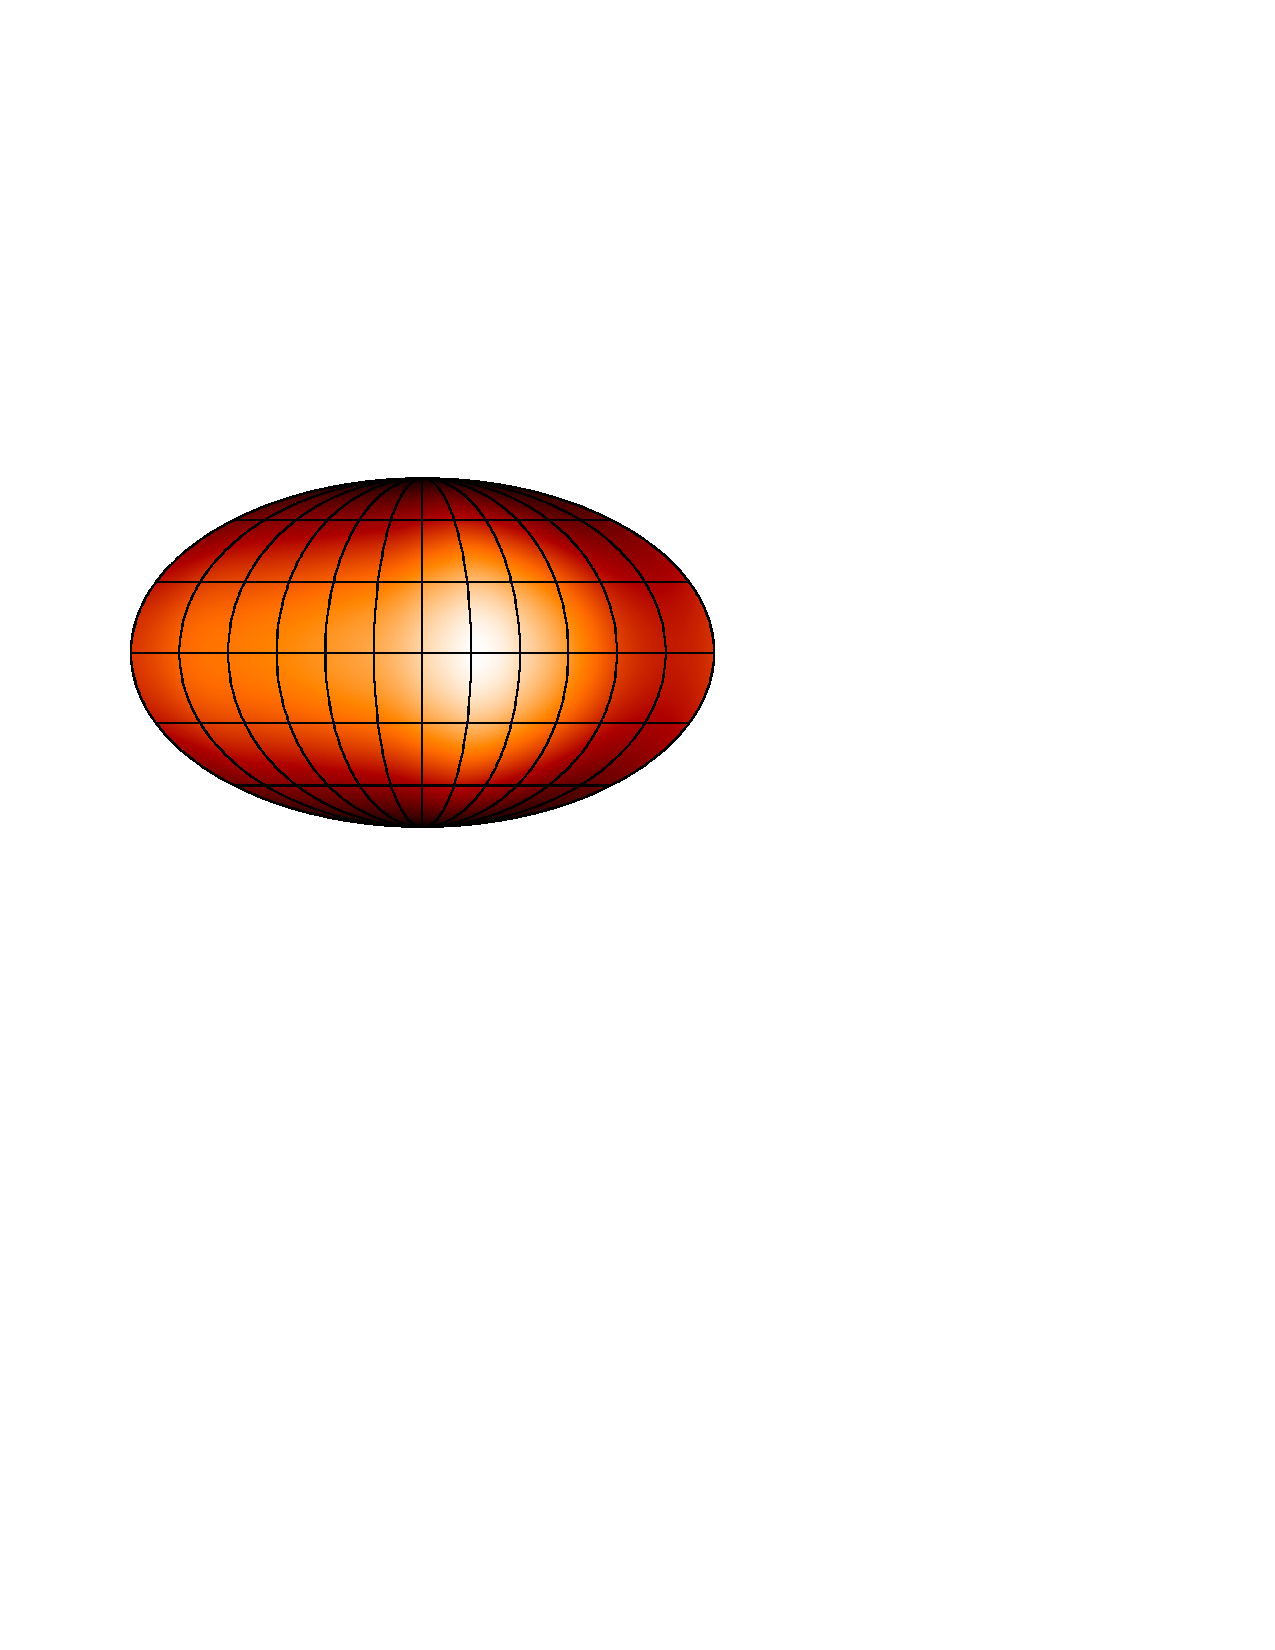
\includegraphics[width=0.4\linewidth]{figures/introduction/knutson_2007_temperature_map_HD_189733b.pdf}
    \caption[Exoplanet phase variations and temperature map.]{Left: Band integrated phase variation of {WASP-43b} from the HST~\citep{stevenson_thermal_2014}.
    The primary transit is inset top right.
    The peak of brightness occurs before the secondary transit.
    Right: Global temperature map of the hot Jupiter HD\,189733b obtained with {Spitzer Space Telescope}~\citep{knutson_map_2007}.
    The hottest point is offset from the sub-stellar point with the day side and night side temperatures around 930\K{} and 650\K{} respectively.}
    \label{fig:phasecurve2014_and_temp_map}
\end{figure}

Secondary transit and phase variations are an extension of the transit method, requiring higher precision to detect the reflection and thermal emission of the exoplanet.
The observed light curve is analysed considering it has two components, not only light emitted from the star but also light from the planet, albeit at a much lower flux level.
To help visualize and discuss the components of exoplanet atmospheres \cref{fig:transits_and_occultations} is provided showing a transiting planet in orbit around a star, in which the planet also passes behind the star causing an occultation.
The planet is shown at several positions of the orbit indicating the proportion of day side and night side observed.
Below the star and planet is a diagram showing the changing flux variation (solid black line) over time, following the orbit.
If the orbital alignment is such that the planet will pass behind the star it will cause an occultation of the planet.
At this point the only light received is from the star alone, creating a baseline stellar measurement.
While during the primary transit there is also a small thermal emission contribution from the night side of the planet, as well as it partially blocking the star.

Throughout the orbit of the planet there is a variation in the planetary flux due to the alternating day/night side of the planet observed.
There are multiple components of the planetary flux, reflection and emission, that can be analysed with multi-band phase curves~\citep[e.g.][]{knutson_characterizing_2009, esteves_optical_2013}.
Optical phase curves will mostly show the reflected light from the day side of the planet, allowing modelling of the atmospheric albedo (fraction of light reflected by the atmosphere), and can provide details on the atmospheric scattering~\citep{madhusudhan_analytic_2012} and aerosol composition~\citep{oreshenko_optical_2016} through the optical phase function (day/night fraction).
Thermal emission of the planet will provide stronger modulation of infrared phase curves and can provide insights into the atmospheres thermal
structure and heat circulation~\citep{goodman_thermodynamics_2009, koll_temperature_2016}.

An example of phase variations in the infrared spectra of {WASP-43b} obtained with the Hubble Space telescope is given in \cref{fig:phasecurve2014_and_temp_map} (left).
The large amplitude of phase variation between the day and night side indicates that the night side is much cooler and there is an inefficient heat circularity from the day to night side.
A planet with an efficient day/night heat distribution mechanism would quickly equalize and have smaller phase variation.
One key observable from \cref{fig:phasecurve2014_and_temp_map} is that the peak of the phase variation is offset from the location of the secondary transit.
The hottest part of the atmosphere does not correspond to the sub-stellar point i.e.\ the point of the planet's surface closest to the star.
This is also observed in surface temperature mapping of the hot Jupiter HD\,189733b obtained with the {Spitzer Space Telescope}~\citep{knutson_map_2007} shown in the right of \cref{fig:phasecurve2014_and_temp_map}.
Simulations of atmospheric circulation models find that this offset is caused by super-rotating equatorial jets which move the location of the hottest point of the planet~\citep[e.g.][and references therein]{heng_atmospheric_2015}.

The point of occultation, at which the planet is completely blocked by the star, enables a baseline measurements for the star to be obtained without the planet.
The depth of the occultation, gives a direct measurement of the relative brightness of the planetary disk if the star-planet radius ratio is known~\citep{winn_transits_2010}.
It is a measure of the flux from the day side of the planet which can indicate the atmospheric reflection and thermal emission of the planet's atmosphere.

Spectra obtained during the occultation will have no planetary signal and can be used remove the stellar component from spectra obtained at other phases to obtain the planetary spectrum.


\subsection{Transmission spectroscopy}
\label{subsec:transmission_spectroscopy}
\begin{figure}
    \centering
    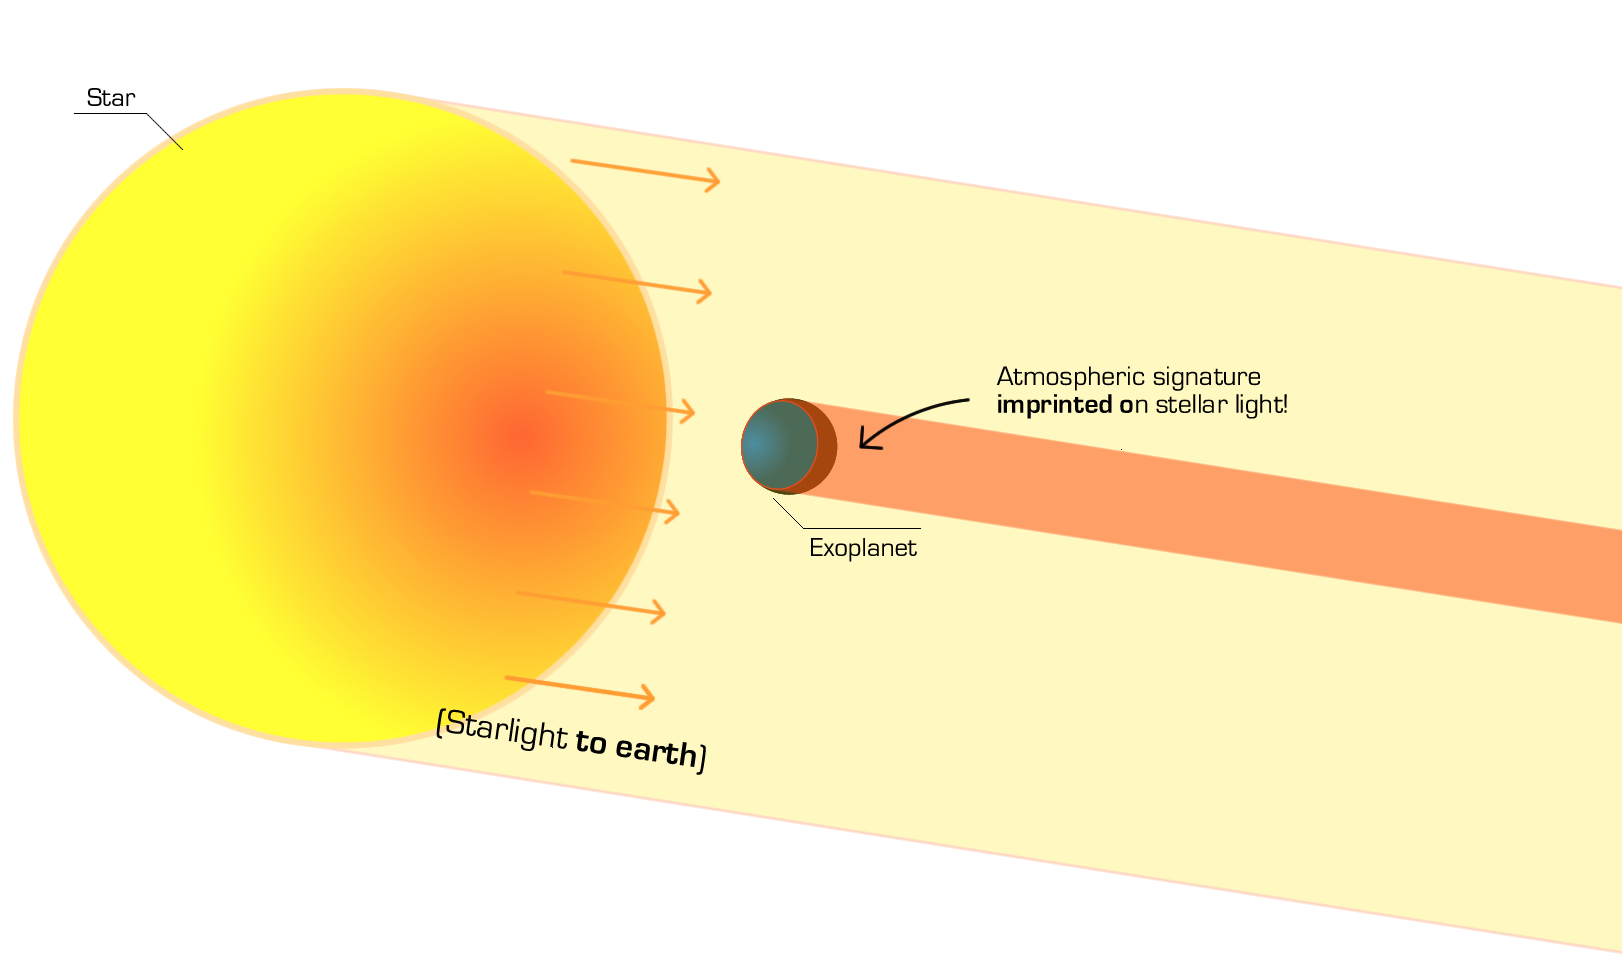
\includegraphics[width=0.65\linewidth]{figures/introduction/transmission_spectroscopy}
    \caption[Transmission spectroscopy diagram.]{Diagram of transmission spectroscopy imprinting the atmosphere of the exoplanet.
    Sourced from \href{http://www.sc.eso.org/~esedagha/research.html}{http://www.sc.eso.org/~esedagha/research.html}}
    \label{fig:transmissionspectroscopy}
\end{figure}

\begin{figure}
    \centering
    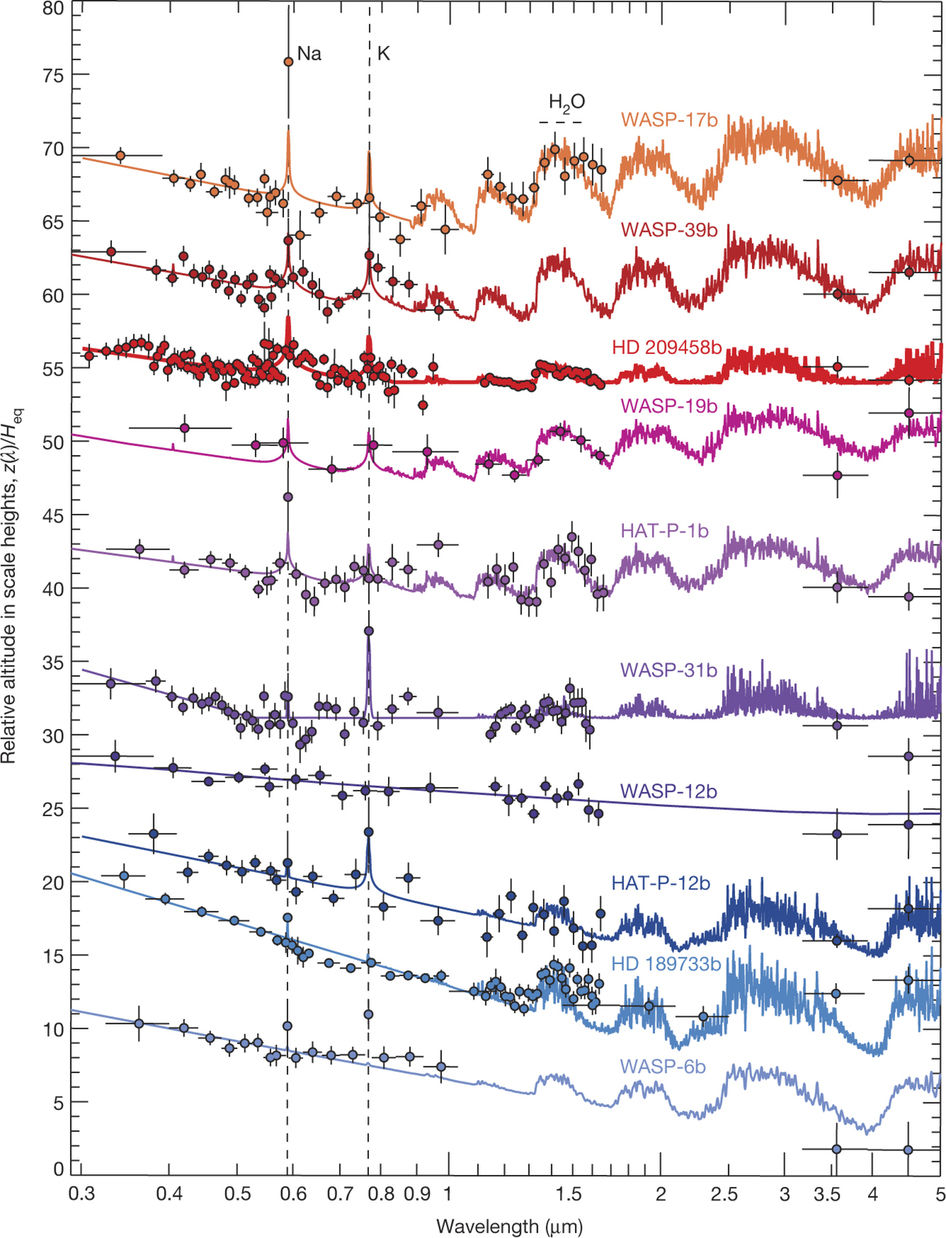
\includegraphics[width=0.6\linewidth]{figures/introduction/transmissionSpec_Sing2016}
    \caption[Transmission spectra for several Hot-Jupiter exoplanets.]{Transmission spectra (dots) for several Hot-Jupiter type exoplanets which increase in the amount of haze and clouds from top to bottom.
    The solid lines indicate the best fit atmospheric models.
    Credit~\citet{sing_continuum_2016}.}
    \label{fig:transmissionspecsing2016}
\end{figure}

When a transiting planet crosses in front of the host star it blocks out light from the star.
However, a small portion of light passes through the atmosphere of the planet as shown in \cref{fig:transmissionspectroscopy}.
The light that passes through the exoplanet atmosphere is partially absorbed, and is faintly imprinted with absorption lines.


In planetary transits, usually defined by their duration and depth, there are degeneracies of the system properties from the transit shape in a single band, for example systems with differently sized planets and stars can have the same \(\frac{\Rp}{\Rstar}\) ratio.
Observing transits in multiple bandpasses (i.e.\ by splitting the spectra observed during transits into several bands) has been shown to break the degeneracies between the stellar radius and the orbital inclination as well as determine the stellar limb darkening~\citep{jha_multicolor_2000, knutson_using_2007}.

The radius of the transiting exoplanet can also appear to change size when observed at wavelengths where there is strong opacity in the atmosphere~\citep[e.g.][]{burrows_radii_2000, seager_theoretical_2000}.
Transits in different wavelength bands will have varying depths, dependant on the opacity of the atmosphere to each band.

The transmission spectra observed with space observatories and ground based high resolution spectrographs has been used to detect several elements and molecules in the atmosphere.
For example \ce{Na}~\citep{charbonneau_detection_2002, redfield_sodium_2008, wyttenbach_spectrally_2015, nikolov_vlt_2016}, \ce{H2O}~\citep{tinetti_water_2007, brogi_carbon_2014}, \ce{CO}~\citep{brogi_carbon_2014, snellen_mass_2018}, \ce{CH4}~\citep{redfield_extrasolar_2010}, \ce{Fe} and \ce{Ti}~\citep{hoeijmakers_atomic_2018}.
The presence of clouds in the atmosphere have also been detected, as they mask the atmospheric constituents as they produce wavelength-independent fluxes~\citep[e.g.][]{barman_clouds_2011, kreidberg_clouds_2014, sing_continuum_2016}.

Transmission spectra for several transiting Hot-Jupiter exoplanets from~\citet{sing_continuum_2016} is shown in \cref{fig:transmissionspecsing2016}.
The amount of haze and clouds present in the atmospheres increases in the spectra shown from the top to bottom.
Hazes are particles produced from chemistry in the atmosphere that results in the formation of involatile solids, while clouds form through the process of condensation and comprise of liquid droplets or ice crystals suspended in the atmosphere. \citet{sing_continuum_2016} defines hazes as having a {Reyleigh}-scattering-like opacity, which could be due to sub-\um{} sized particles, while they define clouds as having a grey opacity, for simplicity.
The spectra near the top have clearer atmospheres, with little or no haze and clouds, show large alkali (\ce{Na} and \ce{K}) and \ce{H2O} absorption. Hazier and cloudier planets lower down the figure have strong optical scattering slopes with narrow alkali lines and have a partially or completely obscured \ce{H2O} absorption. This shows how the transmission spectra can reveal properties if the planetary atmospheres.

\subsection{High resolution spectroscopy}
\label{subsec:high_resolution_spectroscopy}

\begin{figure}
    \centering
    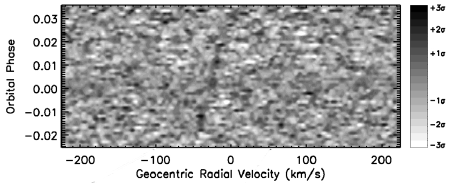
\includegraphics[width=0.7\linewidth]{figures/introduction/snellen2010}
    \caption[Cross-correlation signal from {CRIRES} observations of HD\,209458\,b.]{Cross-correlation signal of {CRIRES} observations during the transit of HD\,209458\,b with a \ce{CO} template.
    Credit~\citet{snellen_orbital_2010}.}
    \label{fig:snellen2010}
\end{figure}

Precise high resolution spectrographs are able to spectrally resolve individual absorption lines, are key to analysing the atmospheres of exoplanets. 
Unfortunately, these are too large and bulky to fly in space, and they would be near impossible to keep in precise alignment during a rocket launch.
The large collecting area of current and future ground based telescopes make high resolution spectroscopy a great contender for obtained high-resolution observations for detecting and exploring exoplanetary atmospheres.

Typically high-resolution and high \snr{} are cross correlated with modelled planetary templates to recover the faint signal of the companion.
This has been most successful in the \nir{} due to the larger planet-to-star flux ratio
notably with CRIRES, with the detection of orbital motion, atmospheric constituents and exoplanetary winds~\citep[e.g.][]{snellen_orbital_2010, dekok_detection_2013, brogi_carbon_2014, brogi_rotation_2016, schwarz_evidence_2015}.
The rotation rate of exoplanets has been achieved by measuring the spectral line broadening~\citep{snellen_fast_2014, brogi_rotation_2016}.
An example of a cross correlated result is given in \cref{fig:snellen2010} showing the shift of the \ce{CO} lines during a transit due to the orbital motion of the planet~\citep{snellen_orbital_2010}.

The spectrum of the star and planet usually cannot be spatially resolved so methods to identify and remove the stellar component are required.
This usually involves constructing a high \snr{} stellar mask from observations, possibly at different phases~\citep[e.g.][]{rodler_weighing_2012}, to subtract from the observed spectra leaving behind the planetary signal.
If the planet is able to be spatially resolved, then a spectrum of the planet could be obtained without stellar contamination~\citep[e.g.][]{snellen_combining_2015}.

High resolution spectroscopy of atmospheres is not limited to transit spectroscopy with detections also possible for non-transiting exoplanets~\citep[e.g.][]{brogi_signature_2012, brogi_carbon_2014,lockwood_nearir_2014, piskorz_evidence_2016}.

An advantage of high-resolution spectra is that it allows the molecular absorption lines of Earth's atmosphere to be resolved.
This way they can be identified and corrected/removed to avoid contamination with the atmosphere of the exoplanet.
 Lower resolution and photometric methods are unable to fully resolve and remove Earth's atmosphere from ground based observations.
